\chapter{Login}

Navigation in the login screen and creation of new accounts. Resetting the password of existing accounts is done through this page. The outlook is depicted below, fields the user to enter are Email-ID, Password, and Admin Key as per requirements.  

\begin{figure}[H]
	\centering
	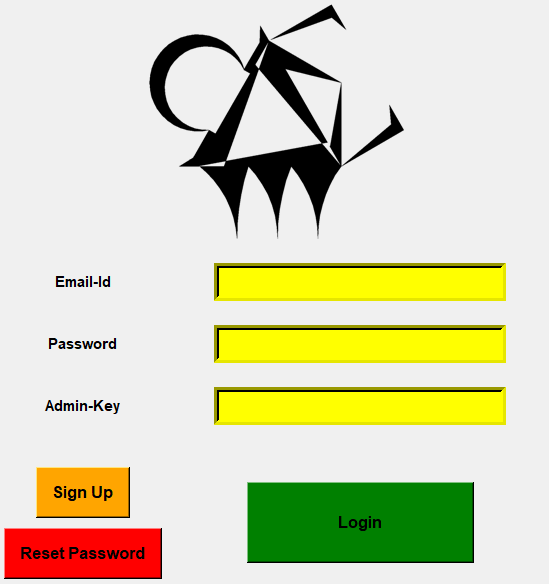
\includegraphics[width=0.6\linewidth]{images/login_page/login_1}
	\label{fig:login1}
\end{figure}

\section{Create New Account}

\begin{itemize}
	\item To create a new account, enter a working Email-ID, and a password of your choice.
	\item Preferably the password must have 8 characters with a special character
	\item The Admin Key is a must, please contact the Admin / Developer of the software in Contact Us
	\item All 3 fields must be entered, now clicking Sign-Up will create the account
	\item Please check verification email to the mail id provided, you can use the new account
\end{itemize}
\begin{figure}[H]
	\centering
	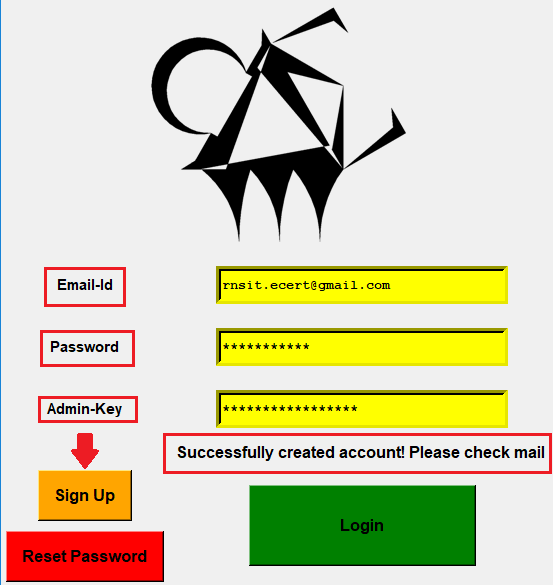
\includegraphics[width=0.6\linewidth]{images/login_page/login_4}
	\label{fig:login4}
\end{figure}

\begin{figure}[H]
	\centering
	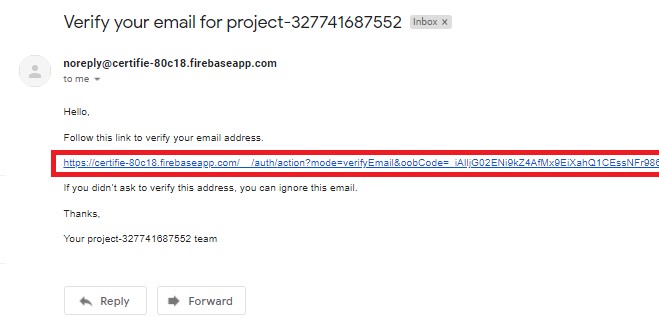
\includegraphics[width=0.9\linewidth]{images/login_page/login_6}
	\label{fig:login6}
\end{figure}

\begin{figure}[H]
	\centering
	
\includegraphics[width=0.95\linewidth]{images/login_page/login_5}
	\label{fig:login5}
\end{figure}

\section{Login with existing Account}

Logging in with existing are newly created account requires a registered Email-ID and Password. 


\begin{figure}[H]
	\centering
	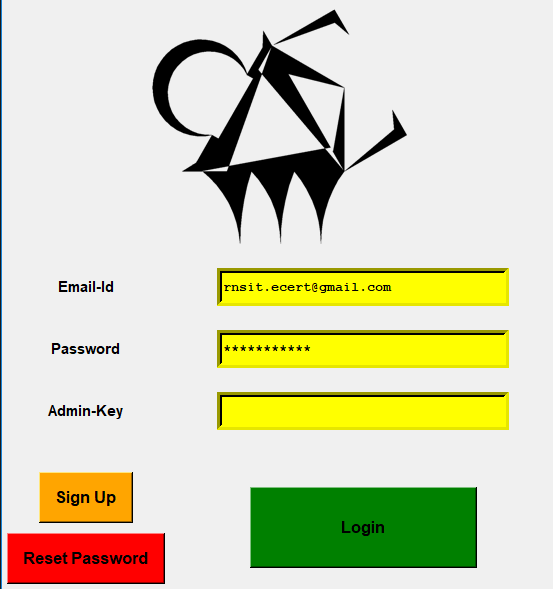
\includegraphics[width=0.45\linewidth]{images/login_page/login_2}
	\label{fig:login2}
\end{figure}

If the Email-ID / Password is erroneous a warning message is displayed to check for the correctness of the Email-ID / Password

\begin{figure}[H]
	\centering
	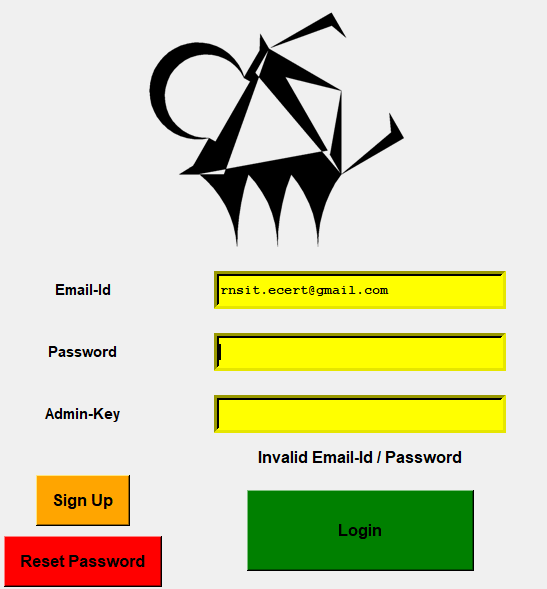
\includegraphics[width=0.45\linewidth]{images/login_page/login_3}
	\label{fig:login3}
\end{figure}

\newpage

\section{Reset Password}

Users can reset the Password in case forgotten. You have to contact the Admin / Developer for the Admin Key.\\

\textbf{Incase Email-ID is forgotten, Sorry we can't help you :(} 

\begin{figure}[H]
	\centering
	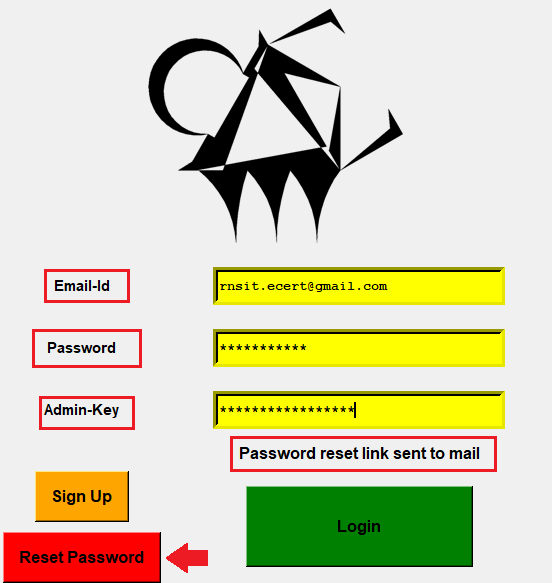
\includegraphics[width=0.6\linewidth]{images/login_page/login_7}
	\label{fig:login7}
\end{figure}







